\documentclass[12pt]{article}
\usepackage[letterpaper, margin=1.3in]{geometry}
\usepackage{amsmath, amssymb, amsthm}
\usepackage{todonotes}
\usepackage[hidelinks]{hyperref}
\usepackage{cleveref}
\usepackage{tikz}
\usepackage{blkarray}
\usepackage{tabularx}
\usetikzlibrary{backgrounds,arrows,automata,positioning,shapes,shapes.geometric,calc, arrows.meta, bending, decorations.pathreplacing}

    \newcolumntype{L}{>{\raggedright\arraybackslash}X}
\newcolumntype{Y}{>{\centering\arraybackslash}X}


\usepackage{witharrows}


\DeclareMathOperator*{\argmax}{argmax}
\DeclareMathOperator*{\argmin}{argmin}

\theoremstyle{definition}
\newtheorem{theorem}{Theorem}[section]
\newtheorem{definition}[theorem]{Definition}
\newtheorem{conjecture}[theorem]{Conjecture}
\newtheorem{proposition}[theorem]{Proposition}
\newtheorem{corollary}[theorem]{Corollary}
\newtheorem{lemma}[theorem]{Lemma}
\newtheorem{claim}[theorem]{Claim}
\theoremstyle{remark}
\newtheorem*{remark}{Remark}
\newtheorem*{example}{Example}

\newenvironment{subproof}[1][\proofname]{%
  \renewcommand{\qedsymbol}{$\blacksquare$}%
  \begin{proof}[#1]%
}{%
  \end{proof}%
}


\title{\Large \textbf{Cooperation Is Provably Required for Success in a Version of the Noisy Iterated Prisoner's Dilemma}}
\author{Arvid Lunnemark \\
\url{arvid@mit.edu}\\ \\
Supervised by: Prof. Michael Sipser}

\begin{document}
\tikzset{elliptic state/.style={draw,ellipse, text centered, text width=10em}}
\tikzstyle{block} = [rectangle, draw, fill=blue!20, 
    text width=5em, text centered, rounded corners, minimum height=4em]

\maketitle

\begin{abstract}
    We introduce a natural model for the iterated prisoner's dilemma in the presence of noise, where strategies are finite automata that at each step have a probability $p$ of making a mistake. This leads us to model the result of two strategies playing against each other as a Markov chain. We prove that for a strategy to be evolutionarily stable in our setup, it has to be cooperative, in the sense that it has to cooperate when playing against a clone of itself. We conjecture that the Pavlov strategy is evolutionarily stable.
\end{abstract}

\section{Introduction}

The prisoner's dilemma is a classic symmetric two-player game, where both players acting in their own best interests leads them to an outcome that is not optimal for either of them. There are two actions: cooperate ($C$) and defect ($D$). The payoffs are awarded according to \cref{fig:prisonersdilemmatable}.

\begin{figure}
    \centering
    \begin{tabularx}{0.8\textwidth}{|c | Y| Y|}
    \cline{2-3}
    \multicolumn{1}{c|}{}
         & Cooperate ($C$) & Defect ($D$) \\ \hline
        Cooperate ($C$) & $R=3 , R=3$ & $S=0, T=5$ \\
         & Reward for mutual cooperation & Sucker's payoff, temptation to defect \\ \hline
        Defect ($D$) & $T=5, S=0$ & $P=1, P=1$ \\
        & Temptation to defect, sucker's payoff & Punishment for mutual defection \\ \hline
    \end{tabularx}
    \caption{The prisoner's dilemma. One player picks a row, the other a column. The payoff of the player picking the row is listed first.}
    \label{fig:prisonersdilemmatable}
\end{figure}

Given the other player's action, a player always maximizes their payoff by choosing to defect, but with both doing so, the players end up in the $(D, D)$ state, which is worse for both than the $(C, C)$ state. The game has been used to model many real-world situations, including countries failing to act to stop climate change, doping in sport, and economic competition.

To make the game more interesting, one can consider playing it multiple times in a row, with multiple players. One might loosely connect this repeated multiplayer game to evolution: why have humans evolved to cooperate with each other? In a seminal paper published in 1980, Axelrod \cite{axelrod1980effective} presented evidence that in a repeated setting with multiple players facing off in a tournament, cooperation can arise as the strategy of choice, even for a selfish player. In particular, the mostly cooperating Tit-for-tat strategy, depicted in \cref{tftfigure}, won his tournament. The idea is that even though Tit-for-tat loses when it plays against defecting strategies, it is being heavily rewarded when it cooperates with other cooperating strategies, resulting in a net advantage for Tit-for-tat.

\begin{figure}
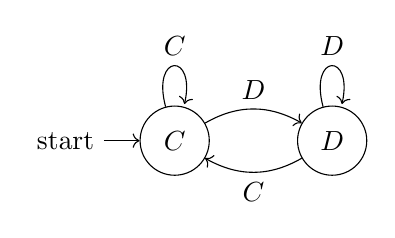
\begin{tikzpicture}[node distance=2cm]
  \node[state,initial] (s_0) {$C$};
  \node[state] (s_1) [right of=s_0] {$D$};

  \path[->] (s_0) edge [loop above] node {$C$} ();
  \path[->] (s_0) edge [bend left] node [above] {$D$} (s_1);
  \path[->] (s_1) edge [loop above] node {$D$} ();
  \path[->] (s_1) edge [bend left] node [below] {$C$} (s_0);
\end{tikzpicture}
  \centering
  \caption{The Tit-for-tat strategy. At any one point, it is in one of two states, taking the action corresponding to the label of that state. It always switches state so as to copy the opponent's last move.}
  \label{tftfigure}
\end{figure}

Clearly, however, the winning strategy in a tournament depends on the composition of strategies in that tournament. If all strategies had been of the type to always defect, Tit-for-tat would not have won the Axelrod tournament. Therefore, follow-up tournaments and simulations have been run, and perhaps surprisingly, most provide further evidence that cooperation is the prevailing strategy, as Axelrod summarized in 1981 in his well-cited book on the topic  \cite{axelrod1981evolution}. There, he also presented an evolutionary model that can be used for analyzing the game: strategies are considered to exist in a population that evolves over time in an evolutionary way (more successful strategies reproduce, and random new strategies are introduced in small numbers). In that context, a strategy is said to be evolutionarily stable if, supposing it controls a large share of the population, it resists being overtaken by any other strategy entering the population in small numbers. That is, populations of evolutionarily stable strategies form the equilibrium states of the evolutionary process, and thus, one may say that the evolutionarily stable strategies are the ``best'' strategies. This characterizes the best strategies without relying on a particular composition of strategies to begin with.

In light of Axelrod's tournaments highlighting the effectiveness of cooperation, it has long been a goal to prove that a cooperating strategy like Tit-for-tat is evolutionarily stable. A few variants on this result has been shown. First, Nowak et al. \cite{nowak2004emergence} showed that in the finitely repeated game, a strategy that always defects is sometimes not evolutionarily stable. Second, Binmore and Samuelson \cite{binmore1992evolutionary} showed that in the infinitely repeated game where strategies are modeled as finite automata where having more states comes at a cost, a strategy needs to cooperate with its clone to be stable. And third, Fudenberg and Maskin \cite{fundenberg1990evolution} showed that a strategy needs to cooperate with its clone to be stable also in the infinitely repeated game in the presence of a certain notion of infinitesimally small noise.

Notably, all these results impose additional restrictions on the setup, and as noted by Fudenberg and Maskin, restrictions are necessary: in the deterministic infinitely repeated game, one could create a strategy that cooperates only with itself — if the opponent ever deviates from what the strategy would do, the strategy resorts to defecting for the rest of the game. This strategy will be evolutionarily stable, but is not necessarily cooperative. 

In this paper, we, like Fudenberg and Maskin, choose the addition of noise as our restriction. In contrast to them, however, we present a model where, at every step, each strategy has a tiny probability $p$ of doing the wrong thing, which is arguably the most natural way of modeling noise. 

In \cref{sectionsetup}, we define the setup of our version of the problem in detail. Then, in \cref{sectionresults}, we state the two main results: a theorem saying that a strategy needs to be cooperative to be evolutionarily stable, and conjecture saying that such evolutionarily stable strategies exist. In \cref{sectionproofs}, we prove our results. Finally, in \cref{sectiondiscussion}, we briefly discuss potential directions for future work.

\section{Setup}
\label{sectionsetup}

In this section we define our setup for the game. In summary, we consider the infinitely repeated prisoner's dilemma played by finite automata in infinite or continuous populations, evolving evolutionarily in the presence of noise.

% \subsection{Formal Definition}

% First, we define the reward function.

\begin{definition}
  The \textit{prisoner's dilemma} is a symmetric two-player game with two actions, cooperate ($C$) and defect ($D$), where, if player 1 selects action $a$ and player 2 selects action $b$, player 1 gets the reward
  \begin{equation*}
    r(a,b) = \begin{cases}
      R &\text{if $a = C, b = C$} \\
      T &\text{if $a = D, b = C$} \\
      S &\text{if $a = C, b = D$} \\
      P &\text{if $a = D, b = D$}
    \end{cases}
  \end{equation*}
  We require $T > R > P > S$ and $2R > T + S$.
\end{definition}

When we study the \textit{iterated} prisoner's dilemma, we want to look at strategies that determine their next move based on the history of previous moves. We restrict ourselves to strategies that can be implemented on a computer with finite memory.

\begin{definition}
  A \textit{strategy} $s$ is a Moore machine (finite automaton with outputs) over the input and output alphabet $\{C, D\}$. 
\end{definition}

Tit-for-tat is depicted as a Moore machine in \cref{tftfigure}.

We will consider strategies in the presence of noise. To model that, we will assume that a strategy has a probability of $1-p$ of following the correct transition, and a probability of $p$ of following the incorrect transition, at every step. Note that this models noise in \textit{perception}. One could also imagine modeling noise in \textit{action taken}, but it is not hard to see that the two are equivalent up to a change in the values of $R, T, S$ and $P$.

We can now begin to define the outcome of two strategies playing against each other in the infinitely repeated game. Markov chains are well suited for this.

\begin{definition}
  Suppose that a strategy $s_1$ plays against a strategy $s_2$. This defines an \textit{$s_1$-$s_2$ Markov chain}, where each state is a tuple $(c_1,c_2)$, with $c_1$ being a state in $s_1$ and $c_2$ a state in $s_2$. The transition probabilities are defined in the obvious way: \begin{equation*}
    p_{(c_1,c_2) \to (c_1', c_2')} = p_{c_1 \to c_1'} \cdot p_{c_2 \to c_2'},
  \end{equation*} where $p_{c_1 \to c_1'}$ is 1 if $s_1$ always transitions from $c_1$ to $c_1'$, 0 if it never does, $1-p$ if the output of $s_2$ at state $c_2$ causes $s_1$ to transition from $c_1$ to $c_1'$, and $p$ if the opposite of that output causes the transition; $p_{c_2 \to c_2'}$ is defined similarly.
\end{definition}

Markov chains naturally lead themselves to the study of limiting cases.

\begin{definition}
  \label{timeaveragedistribution}
  Let $a_0$ be the start state of $s_1$ and $b_0$ the start state of $s_2$. The \textit{time average distribution} of the $s_1$-$s_2$ Markov chain, denoted $\pi$, is the distribution such that \begin{equation*}
    \pi_{c_1, c_2} = E \left[ \text{fraction of time in state $(c_1,c_2)$} \mid \text{start in state } (a_0, b_0)  \right],
  \end{equation*}
  where the expectation is taken over the infinite sequence of states representing a random walk in the Markov chain.
\end{definition}

Note that the time average distribution given a start state always exists, regardless of the structure of the Markov chain.

Now, we can define the payoff that one strategy gets when playing against another one.

\begin{definition}
  \label{payofftimeaverage}
  Let $r(c_1, c_2)$ refer to the reward that $s_1$ gets when $s_1$ takes the action in state $c_1$ and $s_2$ takes the action in state $c_2$. Then, the \textit{payoff that $s_1$ gets when playing against $s_2$} is
  \begin{equation*}
    v_{s_1}(s_2) = \sum_{(c_1,c_2)} \pi_{c_1,c_2} \cdot r(c_1, c_2),
  \end{equation*}
  where the sum is taken over all states $(c_1,c_2)$ in the $s_1$-$s_2$ Markov chain.
\end{definition}

For notational convenience, we may also make $r(c_1, c_2)$ into a vector, denoted by $r$, and write this as the dot product \begin{equation*}
  v_{s_1}(s_2) = \pi \cdot r.
\end{equation*}

That is, the payoff that $s_1$ gets when playing against $s_2$ is simply an average of the reward it gets in each possible state of the Markov chain, weighted by the fraction of time that is spent there.

We're now ready to look at how strategies interact in a multiplayer setting.

\begin{definition}
  A \textit{population} of strategies $P = (S, f)$ is a set $S$ of strategies and a function $f : S \to (0,1]$ such that $\sum_{s \in S} f(s) = 1$, representing the frequency of each strategy in the population.
\end{definition}

\begin{definition}
  The \textit{fitness} of a strategy $s$ in a population $P = (S, f)$ is \begin{equation*}
    F(s) = \sum_{s' \in S} f(s') v_s(s').
  \end{equation*}
\end{definition}

One can think of this as saying that we have infinitely many members of the population, interacting with each other evenly, and that the fitness of a strategy is its expected payoff. Having infinitely many interactions like this justifies the usage of expectation when definining $v_{s_1}(s_2)$.

We can now use the fitness of a strategy to compare it with other strategies in the same population. If a strategy $s_1$ has a higher fitness than another strategy $s_2$, we think of the frequency of $s_1$ as being on the increase, at the expense of the frequency of $s_2$. This is getting us close to how we want to define stable strategies; our next move is looking not only at a single evolutionary step, but the entire evolutionary process.

\begin{definition}
  A strategy $s_1$ is \textit{$\epsilon$-invadable} if there exists a strategy $s_2$ such that in all populations $P$ with $S = \{s_1,s_2\}$ and $f(s_2) \geq \epsilon$, we have 
  \begin{equation*}
    \label{fitnesscond}
    F(s_2) > F(s_1).
  \end{equation*}
\end{definition}

That is, if $s_1$ is $\epsilon$-invadable, there exists a strategy $s_2$ that can start as only a tiny fraction $\epsilon$ of the total population, and consistently have higher fitness than $s_1$, eventually eliminating $s_1$ completely. With this, we can define evolutionary stability.

\begin{definition}
  \label{definitionevolutionarystability}
  A strategy $s_1$ is \textit{evolutionarily stable} if there exists parameters $p_0$ and $\epsilon_0$ with $0 < p_0, \epsilon_0 < 1$, such that for all $p < p_0$, and all $\epsilon < \epsilon_0$, $s_1$ is not $\epsilon$-invadable.
\end{definition}

That is, a strategy $s_1$ is evolutionarily stable if, as the noise probability $p$ goes to 0, it can withstand invasion attempts from any strategy that starts off as a tiny fraction of the population.

% \subsection{Interpretation}

% Having concluded our formal definition of evolutionary stability, it might be helpful to see an example of a concrete setup in which our definitions are applicable and make sense. This will shed light on which parts of our definitions may not be as natural as we would want them to be.

% Consider a square world, inhabited by 

% Consider the following world. 


\section{Results}
\label{sectionresults}

Together, the following theorem and conjecture imply that in the setup described here, mutual cooperation arises as the only stable choice.

\begin{theorem}
  \label{evolutionarystable1}
  Suppose that a strategy $s_1$ is evolutionarily stable. Then \begin{equation*}
  \lim_{p \to 0} v_{s_1}(s_1) = R.
  \end{equation*}
\end{theorem}

\begin{conjecture}
  \label{pavlovtheorem}
  Suppose that $2R > T + P$. Then, the Pavlov strategy, depicted in \cref{pavlovfigure}, is evolutionarily stable.
\end{conjecture}

\begin{figure}
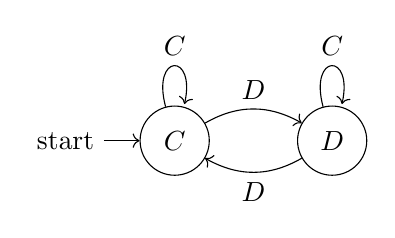
\begin{tikzpicture}[node distance=2cm]
  \node[state,initial] (s_0) {$C$};
  \node[state] (s_1) [right of=s_0] {$D$};

  \path[->] (s_0) edge [loop above] node {$C$} ();
  \path[->] (s_0) edge [bend left] node [above] {$D$} (s_1);
  \path[->] (s_1) edge [loop above] node {$C$} ();
  \path[->] (s_1) edge [bend left] node [below] {$D$} (s_0);
\end{tikzpicture}
  \centering
  \caption{The Pavlov strategy. Similar to but not the same as the Tit-for-tat strategy.}
  \label{pavlovfigure}
\end{figure}


\begin{remark}
  Tit-for-tat, depicted in \cref{tftfigure}, is not evolutionarily stable. 
  When played against itself, it ends up spending just as much time in the defection state as in the cooperation state, because as soon as one mistake is made, it goes into a mutual defection cycle with its clone that is only broken by an additional mistake.
  Thus, $v_s(s)$, where $s$ is Tit-for-tat, is much smaller than $R$, which means that it is not evolutionarily stable by \cref{evolutionarystable1}. Notably, this shows that these results are different, and perhaps stronger, than Fudenberg and Maskin's \cite{fundenberg1990evolution}: while Tit-for-tat is not stable in their model either, their criterion for evolutionary stability does not rule out Tit-for-tat.
\end{remark}


\section{Proofs}
\label{sectionproofs}

In this section, we prove our results from the previous section.

\subsection{The time average distribution}

Before we prove \cref{evolutionarystable1}, we need to understand the mechanisms governing the payoff $v_{s_1}(s_2)$. In this subsection, we prove a series of lemmas that characterize the time average distribution, and in turn $v_{s_1}(s_2)$.

\begin{lemma}
  \label{timeaverageisstationary}
  The time average distribution $\pi$, for a given start state $(a,b)$, is a stationary distribution of the Markov chain. That is, if $M$ is the transition matrix of the Markov chain, we have $M \pi = \pi$.
\end{lemma}

We state this lemma without proof, as it is a fairly standard result. Important to note is that the time average distribution is not necessarily a \textit{unique} stationary distribution, as we do not assume that our Markov chain is ergodic.

\begin{definition}
  A \textit{strongly connected component} of a directed graph is a maximal subgraph where there is a path from every node to every other node.
\end{definition}

\begin{definition}
  An \textit{absorbing component} of a directed graph is a subgraph where there are no edges from vertices inside the component to vertices outside it.
\end{definition}

We may also put both of the terms together and talk about absorbing strongly connected components, which, as shown by the next few lemmas, are useful.

\begin{lemma}
  \label{lemmaabsorbinghasuniquetimeaverage}
  An absorbing strongly connected component has a unique time average distribution. That is, the time average distribution of the component does not depend on the start state (as long as it is inside the component).
\end{lemma}

\begin{proof}
  It is well known that a strongly connected (also known as irreducible) Markov chain has a unique stationary distribution. Since the time average distribution is stationary by \cref{timeaverageisstationary}, it thus also has to be unique.
\end{proof}

\begin{lemma}
  \label{timeaveragedistributiondecomposition}
  Let $\mathcal{A}$ be the set of absorbing strongly connected components of the $s_1$-$s_2$ Markov chain. For every component $S \in \mathcal{A}$, let $\pi^{(S)}$ be its unique time average distribution. Then,
  \begin{equation*}
    \pi = \sum_{S \in \mathcal{A}} P(\text{$s_1$-$s_2$ chain ends up in $S$}) \cdot \pi^{(S)}.
  \end{equation*}
  By $P(s_1\text{-}s_2 \text{ chain ends up in } S)$, we mean the probability of ending up in $S$ given that we start in the initial states of the two strategies and perform a random walk in the Markov chain.
\end{lemma}

\begin{proof}
  Condition all of the following on starting in the start state of $s_1$ and $s_2$. Let $F$ be the fraction of time spent in state $(c_1,c_2)$. If $(c_1,c_2)$ is not in an absorbing strongly connected component, the fraction of time in state $F$ will then be 0. This agrees with what the lemma states. Suppose now that $(c_1,c_2)$ is in an absorbing strongly connected component $S$.
  Let $X$ be the event that the $s_1$-$s_2$ Markov chain ends up in $S$. By the law of total probability, \begin{equation*}
    E[F] = E[F \mid X] \cdot P(X) + E[F \mid \text{not } X] \cdot P(\text{not } X).
  \end{equation*}
   If the random walk on the $s_1$-$s_2$ chain does not end up in the component $S$, but rather in another absorbing strongly connected component, the expected fraction of time in state $(c_1,c_2)$ is clearly 0. Also, note that $E[F \mid X]$ is exactly $\pi^{(S)}_{c_1,c_2}$, and that $E[F]$ is exactly $\pi_{c_1,c_2}$. We thus find that \begin{equation*}
     \pi_{c_1,c_2} = P(\text{$s_1$-$s_2$ chain ends up in $S$}) \cdot \pi^{(S)}_{c_1,c_2}.
   \end{equation*}
   Note that $\pi^{(S')}_{c_1,c_2}$ is 0 for all other absorbing strongly connected components $S'$. With this, we have proved the lemma.
\end{proof}

% Finally, we can characterize the absorbing strongly connected components of the $s_1$-$s_2$ Markov chain in terms of the absorbing SCCs of $s_1$ and $s_2$ separately.

% \begin{lemma}
%   \label{absorbingstronglyconnectedcomponentscartesianproduct}
%   Let $\mathcal{A}_1$ be the set of absorbing strongly connected components of $s_1$, and similarly, let $\mathcal{A}_2$ be the set of absorbing strongly connected components of $s_2$. If $\mathcal{A}$ is the set of absorbing strongly connected components of the $s_1$-$s_2$ Markov chain, then 
%   \begin{equation*}
%     \mathcal{A} = \{H \times K \mid H \in \mathcal{A}_1 \text{ and } K \in \mathcal{A}_2\},
%   \end{equation*}
%   where $A \times B$ is the cartesian product $A \times B = \{(a, b) \mid a \in A \text{ and } b \in B\}$.
% \end{lemma}

% \begin{proof}
%   First, we note that $H \times K$ for all $H \in \mathcal{A}_1$ and $K \in \mathcal{A}_2$ is an absorbing strongly connected component. If there is an edge from $(h,k)$ to $(u,v)$ in the $s_1$-$s_2$ Markov chain, there must, by definition, be an edge from $h$ to $u$ and $k$ to $v$, so $(u,v) \in H \times K$. It is also easy to see that if there is a path 
% \end{proof}

Now that we know more about the time average distribution, we are also interested in proving that the payoff function behaves nicely.

\begin{lemma}
  \label{limitvexists}
  The limit \begin{equation*}
    \lim_{p \to 0} v_{s_1}(s_2)
  \end{equation*}
  exists, for any strategies $s_1$ and $s_2$.
\end{lemma}
\begin{proof}
  By definition, \begin{equation*}
    v_{s_1}(s_2) = \pi \cdot r.
  \end{equation*}

  By \cref{timeaverageisstationary}, $\pi$ is a stationary distribution. In particular, if $M$ is the transition matrix for the $s_1$-$s_2$ Markov chain, then $\pi$ is an eigenvector of $M$ with eigenvalue 1. This implies that $\pi$ is in the nullspace of $M - I$. Thus, we can find $\pi$ by solving for $X$ in $(M - I)X = 0$. If we solve this using Gaussian elimination and back substitution, it is clear that the entries of $\pi$ will be on the form $\frac{f(p)}{g(p)}$ where $f$ and $g$ are polynomials in $p$, since each 
  entry of $M$ is a second-degree polynomial in $p$. This is continuous for all $p$ where $g(p) \neq 0$, and since $g$ will have a finite degree it is therefore continuous in a small right neighborhood of 0. Finally, note that $v_{s_1}(s_2)$ is at least $S$ and at most $T$, which in conclusion means that the limit of $v_{s_1}(s_2)$ as $p$ goes to 0 tends to a finite number, as desired.
\end{proof}

\begin{lemma}
  \label{neverbetterthanr}
  For any strategy $s$,
  \begin{equation*}
    v_{s}(s) \leq R.
  \end{equation*}
\end{lemma}
\begin{proof}
  For notational simplicity, we will let $s_1$ and $s_2$ be two copies of strategy $s$. Then, $v_{s}(s) = v_{s_1}(s_2) = v_{s_2}(s_1)$. By definition, we have
  \begin{equation*}
    v_{s_1}(s_2) = \sum \pi_{c_1,c_2} \cdot r(c_1, c_2)
  \end{equation*}
  and
  \begin{equation*}
    v_{s_2}(s_1) = \sum \pi_{c_2,c_1} \cdot r(c_2, c_1).
  \end{equation*}
  Note that $\pi_{c_1,c_2}$ and $\pi_{c_2,c_1}$ refer to the same state, so we thus have \begin{equation*}
    v_{s_1}(s_2) + v_{s_2}(s_1) = \sum \pi_{c_1,c_2} \cdot (r(c_1,c_2) + r(c_2,c_1))
  \end{equation*}
  which implies that \begin{equation*}
    v_s(s) = \sum \left( \pi_{c_1,c_2} \cdot \frac{r(c_1,c_2) + r(c_2,c_1)}{2} \right).
  \end{equation*}
  Now, note that $r(c_1,c_2) + r(c_2,c_1) \in \{R + R, S + T, T+S, P + P\}$. Since $P < R$ and $T + S < 2R$, we thus find that \begin{equation*}
    v_s(s) \leq \sum \pi_{c_1,c_2} \cdot R = R \sum \pi_{c_1,c_2} = R,
  \end{equation*}
  as desired.
\end{proof}

\subsection{Evolutionary Stability Requires Cooperation}

In this subsection, we prove that evolutionary stability requires that a strategy be cooperating with a clone of itself.

    \begin{proof}[Proof of \cref{evolutionarystable1}]
      Suppose that the strategy $s_1$ is such that it is \textit{not} true that \begin{equation*}
        \lim_{p \to 0 } v_{s_1}(s_1) = R.
      \end{equation*}
      By \cref{limitvexists} and \cref{neverbetterthanr}, this assumption implies that the limit is strictly less than $R$. Define $\gamma = \lim_{p \to 0} v_{s_1}(s_1)$. Then,
      \begin{equation*}
        \gamma < R.
      \end{equation*}
      
      We want to prove that $s_1$ is not evolutionarily stable. 
      
      To do that, we want to prove that for all $p_0, \epsilon_0 \in (0,1)$, there exists $p < p_0$ and $\epsilon < \epsilon_0$, such that $s_1$ is $\epsilon$-invadable. We present a strategy $s_2$ that can invade $s_1$ for all $p$ and $\epsilon$ that are sufficiently small.


      The underlying idea is to construct $s_2$ such that $s_1$ can see no difference between itself and $s_2$, while $s_2$, on the other hand, can. If we succeed in doing so, we will have that $v_{s_1}(s_2) = v_{s_2}(s_1) = v_{s_1}(s_1)$, and will be able to construct $s_2$ such that it always cooperates when it recognizes itself, thereby yielding $v_{s_2}(s_2) = R$. This would give $s_2$ a higher fitness than $s_1$. The rest of this proof executes this plan in detail.

      We create the strategy $s_2$ as follows. First, we copy all of $s_1$ into $s_2$. Let $\mathcal{A}_1$ be the set of
       absorbing strongly connected components of $s_1$. The key idea, now, is to replace each original absorbing strongly connected component $H \in \mathcal{A}_1$ with a new absorbing component $K_H$, which has the capability of distinguishing between itself and $s_1$.

      We now describe how to construct $K_H$ for each $H$. \Cref{c2flowchart} shows the high-level construction of $K_H$.
       All of the steps succeed with probability $1 - O(p)$. The first step makes sure that $K_H$ does not deviate from $s_1$ at all
        until $s_1$ has reached an absorbing strongly connected component. 
       Once $s_1$ is in an absorbing strongly connected component, it cannot escape, and $s_2$ can also force it to end up in any of the states in the component, which means that even if $s_1$ after this point ``figures out'' that it is not playing against itself anymore, there's nothing it can do about it.
      The second step in the construction of $K_H$ makes sure that if $s_2$ is playing against itself, it is in sync with its clone; that is, with probability $1 - O(p)$, both copies of $s_2$ will transition to the third component at the exact same time (although not necessarily in the same $K_H$). 
      The third step figures out what action $s_1$ would take at some large finite time $T$. 
      Then, $K_H$ outputs the exact opposite action at time $T$. 
      At that point, if its opponent outputs $s_1$'s expected action, it wants to transition into the absorbing strongly connected component $H_\text{copy}$, which is just an exact copy of $H$, but if its opponent outputs the opposite of that action, it has successfully distinguished its opponent from $s_1$ and thus enters an always cooperating state.
      Before transitioning into $H_\text{copy}$, $s_2$ makes sure that $s_1$ is in a state that is beneficial for $s_2$.

      \begin{figure}
        \centering
        \begin{tikzpicture}[node distance=0.9cm,initial text=]
          \node[elliptic state, initial, initial where=above] (c_0) {1. Wait until $s_1$ is in an absorbing SCC, while simulating $H$.};
          \node[elliptic state] (c_1) [below=of c_0] {2. Sync up with $s_2$.};
          \node[elliptic state] (c_3) [below=of c_1] {3. Figure out what action that $s_1$ will take right after this.};
          \node[state] (c_4) [below left=of c_3] {$C$};
          \node[state] (c_5) [below right=of c_3] {$D$};
          \node[state] (c_6) [below=of c_5] {$C$};
          \node[elliptic state] (c_7) [below=of c_4] {4. Force $s_1$ into a good state.};
          \node[elliptic state] (c_8) [below=of c_7] {$H_\text{copy}$ \\(an exact copy of $H$)};


          \path[->] (c_0) edge (c_1);
          \path[->] (c_1) edge (c_3);
          \path[->] (c_3) edge node [above left] {$s_1$ will take $D$} (c_4);
          \path[->] (c_3) edge node [above right] {$s_1$ will take $C$} (c_5);
          \path[->] (c_4) edge node [below, pos=0.1] {$C$} (c_6);
          \path[->] (c_5) edge node [right] {$D$} (c_6);
          \path[->] (c_4) edge node [left] {$D$} (c_7);
          \path[->] (c_5) edge node [below, pos=0.1] {$C$} (c_7);
          \path[->] (c_6) edge [loop right] (c_6);
          \path[->] (c_7) edge (c_8);
          % \path[->] (c_0) edge node [above right] {$\bar{\alpha}$} (c_1);
          % \path[->] (c_1) edge [loop right] node [right] {$C,D$} ();
          % \path[->] (c_0) edge node [above left] {$\alpha$} (c_prime);
          % \path[->] (c) edge node [below left] {$\alpha$} (c_prime);
        \end{tikzpicture}
        \caption{High-level construction of $K_H$, the absorbing component replacing $H$ in the creation of $s_2$ in the proof of \cref{evolutionarystable1}. Note that $K_H$ contains exactly 2 absorbing strongly connected components. SCC is short for strongly connected component.}
        \label{c2flowchart}
      \end{figure}
      
      This concludes the high-level construction of $s_2$. We now want to prove that this $s_2$ can in fact invade $s_1$. To do that, we will first assume that the below four lemmas are correct, that is, that the construction is possible and works as specified, and then finish the proof of our theorem using those assumptions. Once that's done, we will prove the four lemmas.

      \begin{lemma}
        \label{claimcanwaitfors1}
        We can construct a non-absorbing component with behavior indistinguishable from the behavior of component $H$, such that when we leave the component, $s_1$ will be in an absorbing strongly connected component with probability $1 - O(p)$.
      \end{lemma}

      \begin{lemma}
        \label{claimcansyncs2}
        We can construct a non-absorbing component placed after the first component, such that if $s_2$ plays against itself, both clones transition from the second component to the third component of their respective $K_H$ at the exact same time, with probability $1 - O(p)$.
      \end{lemma}

      \begin{lemma}
        \label{claimcanfigureout}
        We can construct a non-absorbing component with a finite number of maximum steps that, supposing that $s_2$ plays against $s_1$, can figure out what action $s_1$ will take at the exact timestep following the transition out of the component. This component is the same for all $H$.
      \end{lemma}

      \begin{lemma}
        \label{claimcanforcegoodstate}
        We can construct a non-absorbing component placed after the third component that, supposing that $s_2$ plays against $s_1$, can transition into any given absorbing strongly connected component $S$ in the $s_1$-$s_2$ chain that is a subset of $H_\text{copy} \times H'$ where $H'$ is the absorbing strongly connected component that $s_1$ is in.
      \end{lemma}

      We now finish our proof, starting with a lemma concerning the payoffs.

      \begin{lemma}
        \label{claimpayoffs}
        Given the above construction of $s_2$, the payoffs are as follows.
      \begin{align*}
        v_{s_1}(s_1) &= \gamma \pm O(p), \\
        v_{s_2}(s_2) &= R \pm O(p),
      \end{align*}
      and either
      \begin{align*}
        \lim_{p \to 0} v_{s_2}(s_1) > \gamma,
      \end{align*}
      or
      \begin{align*}
        v_{s_2}(s_1) = \gamma \pm O(p) \text{ and }
        v_{s_1}(s_2) \leq \gamma \pm O(p).
      \end{align*}
      \end{lemma}
      \begin{subproof}
        By our definition of $\gamma$, we have that $v_{s_1}(s_1) = \gamma \pm O(p)$.

        Consider now the $s_2$-$s_2$ Markov chain. By \cref{claimcansyncs2}, both clones will transition into the third component at the exact same time. The third component spends only a finite amount of time by \cref{claimcanfigureout}, and is the same regardless of which $K_H$ the strategies are in. Thus, after leaving the third component of $K_H$, if no mistakes have happened since leaving the second component, both clones of $s_2$ will be in exactly corresponding states, since they will always mirror each other. This happens with probability at least $(1-p)^N$ where $N$ is the finite number of states in the third component, and thus with probability $1 - O(p)$. Thus, in the identifying stage, both clones will output the same action, and as we can see in \cref{c2flowchart}, they will then both transition to the always cooperating state with probability $1 - O(p)$. Therefore, $v_{s_2}(s_2) = R \pm O(p)$.

        Consider now the case of $s_1$ playing against $s_2$. Suppose that $s_2$ ends up in the absorbing component $K_H$. By \cref{claimcanwaitfors1}, with probability $1 - O(p)$, $s_2$ is indistinguishable from $s_1$ until $s_1$ reaches an absorbing strongly connected component, which we call $H'$.         
        This means that the probability of reaching the absorbing component $H' \times K_H$ of the $s_1$-$s_2$ Markov chain, is up to a factor of $1 - O(p)$ the same as if we had not replaced $H$ by $K_H$ in $s_2$, which is just the probability of reaching the absorbing component $H' \times H$ in the $s_1$-$s_1$ Markov chain. Thus, 
        \begin{equation*}
          P(\text{$s_1$-$s_2$ ends up in $H' \times K_H$}) = (1 - O(p)) P(\text{$s_1$-$s_1$ ends up in $H' \times H$})
        \end{equation*}
        Now, by \cref{claimcanfigureout}, the probability that $s_2$ enters the absorbing strongly connected component $H_\text{copy}$ after having gotten to $K_H$ is $1 - O(p)$ when playing against $s_1$. Thus,
        \begin{equation}
          \label{equationhhcopy}
          P(\text{$s_1$-$s_2$ ends up in $H' \times H_\text{copy}$}) = P(\text{$s_1$-$s_1$ ends up in $H' \times H$}) \pm O(p).
        \end{equation}
        % Let $C_H$ be the always cooperating absorbing state of $K_H$. Then, this equation implies that 
        % \begin{equation}
        %   \label{equationhch}
        %   P(\text{$s_1$-$s_2$ ends up in $H' \times C_H$}) = O(p).
        % \end{equation}
        By \cref{claimcanforcegoodstate}, $s_2$ can choose to end up in any absorbing strongly connected component $S_{H', H}$ that is a subset of $H' \times H_\text{copy}$, with probability $1 - O(p)$. 
        Naturally, $s_2$ chooses an $S_{H', H}^*$ as follows: among the $S$ that have the maximum payoff for $s_2$, in the limit as $p$ goes to 0, we choose the one the minimizes the payoff for $s_1$.
        Let $v_{s}(S)$ denote the payoff that strategy $s$ achieves in the absorbing strongly connected component $S$ of the Markov chain. Then,
        \begin{equation}
          \label{imtoootired}
          v_{s_2}(S_{H', H}^*) \geq \sum_{S} P(\text{$s_1$-$s_1$ ends up in $S$} \mid \text{$s_1$-$s_1$ ends up in $H' \times H$}) \cdot v_{s_1}(S) \pm O(p)
        \end{equation}
        since the right hand side is a weighted average of $v_{s_1}(S)$, which is the same as $v_{s_2}(S)$ in this case, which is what we maximized over when we chose $S_{H', H}^*$. Also, since $s_2$ could ensure with probability $1 - O(p)$ that the Markov chain enters $S_{H',H}^*$ (by \cref{claimcanforcegoodstate}), we have
        \begin{equation}
          \label{eqshh}
          P(\text{$s_1$-$s_2$ ends up in $S_{H',H}^*$}) = P(\text{$s_1$-$s_2$ ends up in $H' \times H_\text{copy}$})  \pm O(p).
        \end{equation}
        Also, as a consequence, the collection of $S_{H,H'}^*$ for all $H$ and $H'$ become the only absorbing strongly connected components with probabilities of ending up in them greater than $O(p)$.

        Now, let $\mathcal{A}$ be the set of absorbing strongly connected components of the $s_1$-$s_1$ chain, and let $\mathcal{B}$ be the set of absorbing strongly connected components of the $s_1$-$s_2$ chain. We can now calculate $v_{s_2}(s_1)$.

        % By definition, $v_{s_1}(s_1) = \gamma$. By \cref{timeaveragedistributiondecomposition}, the time average distribution of the $s_1$-$s_1$ Markov chain $\pi$ is \begin{equation*}
        %   \pi = \sum_{(C_1, C_1') \in \mathcal{C}_1 \times \mathcal{C}_1} p_{(C_1, C_1')} \cdot \pi^{(C_1, C_1')}
        % \end{equation*}
        % When creating $s_2$, we replaced each $C_1$ by a $C_2$, containing two absorbing strongly connected components: a copy of $C_1$, which we call $C_{1, \text{copy}}$ and the always cooperating $C_c$. This means that the condensation of the $s_1$-$s_2$ Markov chain is the same as the condensation of the $s_1$-$s_1$ Markov chain, except that each absorbing strongly connected component has been replaced by two. That is, the absorbing strongly connected component $(C_1, C_1')$ of the $s_1$-$s_1$ chain has become both $(C_1, C_{1, \text{copy}})$ and $(C_1, C_c)$ in the $s_1$-$s_2$ chain. Then, we find by our construction, that 
        % \begin{align}
        %   \label{c1c1copy}
        %   p_{(C_1, C_{1, \text{copy}})} &= (1 - O(p)) p_{(C_1, C_1')} \\
        %   p_{(C_1, C_c)} &= O(p) p_{(C_1, C_1')}
        % \end{align}
        % This equation is true because when $s_2$ plays against $s_1$, it identifies the action $A$ that $s_1$ will take at time $A$ with probability $(1 - O(p))$, and upon seeing that transitions to $C_{1, \text{copy}}$ with probability $(1-p)$.

        \begin{align*}
          \WithArrowsOptions{displaystyle}
          \begin{WithArrows}
          v_{s_2}(s_1) &= \sum_{S \in \mathcal{B}} P(\text{$s_1$-$s_2$ ends up in $S$}) \cdot v_{s_2}(S) \\
          &= \sum_{S_{H',H}^*} P(\text{$s_1$-$s_2$ ends up in $S_{H', H}^*$}) \cdot v_{s_2}(S_{H', H}^*) \pm O(p) \Arrow{\cref{eqshh}} \\
          &= \sum_{S_{H',H}^*} P(\text{$s_1$-$s_2$ ends up in $H' \times H_\text{copy}$}) \cdot v_{s_2}(S_{H', H}^*) \pm O(p) \Arrow{\cref{equationhhcopy}} \\
          &= \sum_{S_{H',H}^*} P(\text{$s_1$-$s_1$ ends up in $H' \times H$}) \cdot v_{s_2}(S_{H', H}^*) \pm O(p) \Arrow{\cref{imtoootired}}\\
          &\geq \sum_{S \in \mathcal{A}} P(\text{$s_1$-$s_1$ ends up in $S$}) \cdot v_{s_1}(S) \pm O(p)\\
          &= v_{s_1}(s_1) \pm O(p)
          \end{WithArrows}
        \end{align*}
        Thus, we have that $v_{s_2}(s_1) \geq \gamma \pm O(p)$. Suppose that $v_{s_2}(s_1) = \gamma \pm O(p)$. Then, we must have equality in \cref{imtoootired} for all $H$ and $H'$, which means that all $S$ were equally good for $s_2$, in which case we chose $S_{H',H}^*$ to minimize the payoff for $s_1$. Following through with the exact same argument as above, but flipping the inequalities, we then find that $v_{s_1}(s_2) \leq \gamma \pm O(p)$. This proves the lemma.
      \end{subproof}

      Given \cref{claimpayoffs}, we simply compute $F(s_2) - F(s_1)$, which we want to show is greater than 0. We have two cases. First, we assume that $\lim_{p \to 0} v_{s_2}(s_1) > \gamma$. Let $\lim_{p \to 0} v_{s_2}(s_1) = \beta$. Then,
      \begin{align*}
        F(s_2) - F(s_1) &= \\
        &= (1 - \epsilon) \cdot v_{s_2}(s_1) + \epsilon \cdot v_{s_2}(s_2) - (1 - \epsilon) \cdot v_{s_1}(s_1) - \epsilon \cdot v_{s_1}(s_2) \\
        &= (1 - \epsilon) (\beta \pm O(p)) + \epsilon (R \pm O(p)) - (1-\epsilon) (\gamma \pm O(p)) - \epsilon (v_{s_1}(s_2) \pm O(p)) \\
        &= (1 - \epsilon) (\beta - \gamma) + \epsilon(R - v_{s_1}(s_2)) \pm O(p)
      \end{align*}
      Here, we can make $\epsilon$ and $p$ small enough such that this becomes positive, since $\beta - \gamma > 0$. Now, in the second case, we assume that $v_{s_2}(s_1) = \gamma \pm O(p)$ and $v_{s_1}(s_2) \leq \gamma \pm O(p)$. Then,
      \begin{align*}
        F(s_2) - F(s_1) &= \\
        &= (1 - \epsilon) \cdot v_{s_2}(s_1) + \epsilon \cdot v_{s_2}(s_2) - (1 - \epsilon) \cdot v_{s_1}(s_1) - \epsilon \cdot v_{s_1}(s_2) \\
        &\geq (1 - \epsilon) (\gamma \pm O(p)) + \epsilon (R \pm O(p)) - (1-\epsilon) (\gamma \pm O(p)) - \epsilon (\gamma \pm O(p)) \\
        &\geq \epsilon (R - \gamma) \pm O(p)
      \end{align*}
      We know that $R - \gamma > 0$ by our initial assumption. Here, we can make $p$ small enough such that this becomes positive.
      
      In conclusion, our constructed $s_2$ has higher fitness than $s_1$. This proves that $s_2$ can invade $s_1$, and thus, that $s_1$ is $\epsilon$-invadable some values of $p < p_0$ and some $\epsilon < \epsilon_0$. In conclusion, then, $s_1$ is not evolutionarily stable, which concludes the proof of \cref{evolutionarystable1}.

    \end{proof}

      We now return to the four lemmas that we left out, which detail the construction of $s_2$.

      \begin{proof}[Proof of \cref{claimcanwaitfors1}]

        Let $T_1$ be a random variable designating the time at which $s_1$ transitions into an absorbing strongly connected component, counting from the time that $s_2$ entered $K_H$. (In particular, if $s_1$ is already in an absorbing strongly connected component, $T_1 = 0$.)
        Let $T_2$ be a random variable designating the time at which $s_2$ transitions out of component 1 in $K_H$.
        To prove our lemma, we want to prove that with probability $1 - O(p)$, $T_1 \leq T_2$, and that during all the time that we are in component 1 of $K_H$, the output of $s_2$ is indistinguishable from $H$.

        First, we deal with the indistinguishability part. We create the component by copying $H$. Next, we define a new graph $W$, that we will design in the subsequent paragraphs, which will wait for $s_1$ to get into an absorbing component. This graph will have edges defined with the labels $C$ and $D$, but will have no outputs at its states. The graph $W$ will also have one designated end state. We will then construct our component 1 for $K_H$ by replacing every state $h \in H$ with a copy of $W$ that we call $W_h$. There will be a $C$ edge from node $u \in W_h$ to node $v \in W_{h'}$ if and only if there is a $C$ edge from $h$ to $h'$ in $H$, and from $u$ to $v$ in $W$. Similarly for the $D$ edge. This is commonly known as the Kronecker or tensor product of the graphs $H$ and $W$. The output at every state $u \in W_h$ is the same as the output of $h$. For the end state $e \in W_h$ for each $h$, we will add an edge labeled both $C$ and $D$, transitioning out of this component and into component 2.

        It is clear that as long as we don't transition out of this component, the Kronecker product will ensure that the output will be indistinguishable from $H$. We now want to design $W$ such that $T_1 \leq T_2$ with high probability.
        
        Let $d$ be the maximum length of a path from any state in $s_1$ to its closest absorbing strongly connected component. Then, for each state in $s_1$, there is a sequence of perceived inputs of length $\leq d$ (the \textit{special sequence} for that state), such that $s_1$ upon seeing that sequence ends up in an absorbing strongly connected component. For all states, the probability that $s_1$ 
        perceives its special sequence is $\geq p^d$, since, in the worst case, $s_1$ would need to make a mistake on exactly all 
        inputs to perceive the special sequence. That means that at any single point in time, there is a probability $\geq p^d$ that $s_1$ 
        will go into an absorbing strongly connected component within the subsequent $d$ moves. Consider the geometric random variable $X_1 = d + \operatorname{Geom} (p^d)$. We may see $X_1$ as some sort of upper bound to $T_1$.

        We now describe the construction of $W$. Consider a state $c_1 \in s_1$ and a state $h \in H$, and suppose that we let them evolve with no mistakes happening at all. Then, the outputs of $s_1$ will form an infinite string $l(c_1, h)$. Let there be $|s_1|$ states in $s_1$ and $|H|$ states in $H$. Now, create a string $l^*$ of length $|s_1| \cdot |H|$, which differs in at least 1 place from each $l(c_1,h)$.\footnote{This is the famous technique of diagonalization.} Thus, if $s_1$ ever outputs the string $l^*$ when we are in this component, we know that at least one mistake has occurred, somewhere. Consequently, the probability that, at each timestep, $l^*$ will be perceived by $s_2$ as the next sequence of outputs of $s_1$ is $\leq p$. 
        If we repeat $l^*$ for $d+1$ times to form $(l^*)^{d+1}$, the probability that that string is perceived by $s_2$ as the next sequence of outputs of $s_1$ is $\leq p^{d+1}$.
        Now, create $W$ as follows: it is a chain of states $w_1,w_2,\ldots,w_{(d+1)|l^*|+1}$ where $w_i$ transitions to $w_{i+1}$ on seeing the $i$th character of the string $(l^*)^{d+1}$; $w_i$ transitions to $w_1$ otherwise. $w_{(d+1)|l^*|+1}$ is the designated end state of $W$. Now, it is clear that each step, the probability that we will reach the end state in the next $(d+1)|l^*|+1$ steps is $\leq p^{d+1}$. Consider the geometric random variable $X_2 = (d+1)|l^*| + 1 + \operatorname{Geom} (p^{d+1})$. We may see $X_2$ as a lower bound to $T_2$.

        We now claim that the probability that $X_1 \leq X_2$ is $1 - O(p)$, where $X_1$ and $X_2$ are independent. It suffices to show that $\operatorname{Geom}(p^d) \leq \operatorname{Geom}(p^{d+1})$ with high probability, and it further suffices to show that $\operatorname{Geom}(x) > \operatorname{Geom}(px)$ with probability $O(p)$, for some arbitrary $x$. This is easy to show. Consider the geometric variable with parameter $px$ to consist of first an event of probability $x$ happening, and then that counts as a real success with a probability $p$. Then, when comparing the two geometric variables, it is clear that both are equally likely to have an event of probability $x$ happening first. Thus, with probability $\frac{1}{2}$, $\operatorname{Geom}(x)$ gets the first real success, with probability $\frac{1}{2} \cdot p$, $\operatorname{Geom}(px)$ gets the first real success, and with probability $\frac{1}{2} (1 - p)$, we saw a fake success and will continue waiting for the next potential success. Clearly, then, $\operatorname{Geom}(x)$ will get the first success with probability $\frac{1}{2} / (\frac{1}{2} + \frac{1}{2}p)$. Thus, $\operatorname{Geom}(px)$ will get the first success with probability $p / (1 + p) = O(p)$, which is exactly what we wanted to show.

        This concludes the proof that component 1 is such that with probability $1 - O(p)$, $s_1$ will have reached an absorbing strongly connected component before $s_2$ continues to component 2 of $K_H$.
      \end{proof}

      \begin{proof}[Proof of \cref{claimcansyncs2}]
        This construction is relatively simple. It is a chain of states where each state transitions to the next on both input $C$ and $D$ (that is, deterministically). Let $l_H^*$ be the string used in the proof of \cref{claimcanwaitfors1} for component $H$. Let $L = \sum_{H} (d+1) | l_H^* |$. Then, the outputs of the first $L$ states form the string $l_H^*$ repeated $d+1$ times, for all $l_H$. The following $L+1$ states always output $D$. This is followed by one last state outputting $C$. The $C$ state has a transition into itself on input $D$, and out of this component (to component 3 of $K_H$) on input $C$.

        Suppose that $s_2$ plays against a clone $s_2'$ of itself, and that $s_2$ enters an absorbing component $K_H$ first. Then, by \cref{claimcanwaitfors1}, using the fact that $s_2'$ is a copy of $s_1$ before it reaches an absorbing component, $s_2$ will not enter component 2 of $K_H$ until $s_2'$ enters an absorbing component $K_{H'}$, with probability $1 - O(p)$. When $s_2$ enters component 2, it will at some point output the entirety of the string $l_{H'}^*$. With probability $1 - O(p)$, $s_2'$ will then, by our construction of component 1, enter component 2. That is, $s_2'$ enters the first part of component 2 before $s_2$ leaves the first part of component 2, which means that $s_2$ is at most $L$ steps ahead of $s_2$. This means that $s_2'$ will be in the defection part of the chain when $s_2$ reaches the cooperation state. Assuming no mistakes, then, $s_2$ will wait until $s_2'$ also reaches the cooperation state, at which point they will both simultaneously leave the component. This happens with probability $1 - O(p)$, as desired.
      \end{proof}

      \begin{proof}[Proof of \cref{claimcanfigureout}]
        
          Let $\mathcal{A}_1$ be the set of all absorbing strongly connected components in $s_1$.
           Let $L$ be the set of all tuples of $(H, h)$ where $H \in \mathcal{A}_1$ and $h$ is a possible state of $H$. 

        The third component is implemented as follows. When we talk about ``at compile time'' we refer to when we construct the finite automaton.
        \begin{enumerate}
          \item Iterate over every pair of tuples $(H,h)$ and $(H', h')$ in $L$:
          \begin{enumerate}
            \item At compile time, we know what actions have been taken so far in this component, and thus know, if $s_1$ were in $H$ in state $h$ when $s_2$ started out this component, the state $g$ that $s_1$ is in now, with high probability. Similarly supposing that $s_1$ were in $H'$ in state $h'$ when $s_2$ started out this component, we know the state $g'$ where $s_1$ would be now.
            \item At compile time, we also know whether there exists an input string $w$ such that $s_1$ starting in state $g$ perceiving $w$ produces a different output sequence than if it started in state $g'$, following only $1-p$ transitions.
            \item If no such $w$ exists, continue the loop here.
            \item If such a $w$ exists, then output $w$ deterministically here. Determine if the sequence of perceived actions corresponds to what would be expected from $(H,h)$ or from $(H', h')$.
          \end{enumerate}
        \end{enumerate}
        In the end, there will be a subset $U$ of $L$ that corresponds to all tuples $(H,h)$ that corresponded to the perceived sequence of actions in each comparison it was part of. By the way the loop is constructed, all $(H,h)$ in $U$ will produce the same high probability output on any input string; for our purposes, we can therefore just pick one canonical $(H,h)$ from $U$.

        Note that when we implement this procedure on a finite automaton, it becomes a large decision tree, which means that in the end, there will be one branch for each canonical $(H, h)$, and we will be in one corresponding to where $s_1$ actually started off in the beginning of this component with probability $1 - O(p)$. In each such branch, we know, at compile time, which state $s_1$ is in at the end of the branch, and thus know what output that $s_1$ will have in the next step, with probability $1 - O(p)$. This is exactly what we wanted, so we transition out of component 3.
      \end{proof}


      \begin{proof}[Proof of \cref{claimcanforcegoodstate}]
        Note that an absorbing strongly connected component $S$ of the $s_1$-$s_2$ chain that is a subset of $H_\text{copy} \times H'$ can be gotten to by making $s_1$ transition to some state $h_1$ and $s_2$ transition to some state $h_2 \in H_\text{copy}$ where $(h_1, h_2) \in S$. This is simple. Note that $s_1$ is in a strongly connected component already, and that $s_2$ knows, by the previous component, which state $s_1$ is in. Thus, $s_2$ knows the path for $s_1$ to get to $h_1$, and can just output that. Then, $s_1$ will be in $h_1$, and $s_2$ can simply transition to $h_2$. This proves the lemma.
      \end{proof}


    %   \todo{KEY IMPORTANT DETAIL: we need to say that at a large finite $T$ then $s_1$ will be within an absorbing strongly connected component. probably need to look at all possible starting states of all possible ASCCs, not only every ASCC. uhhhhhhhhhhhh also need to modify our language a little bit to think about the fact that absorbing strongly connected components of $s_2$ actually DO AFFECT the condensation probabilities. however, since $C_2$ behaves as $C_1$ for many steps, it won't affect it meaningfully. }

    % \begin{proof}
    %   \begin{claim}
    %     Suppose that there are no mistakes, i.e., that $p = 0$. We can create a $C_2$ such that 
    %   \end{claim}
      
    %   First, copy the entire $s_1$ machine into $s_2$. Suppose that the state corresponding to the start state of $s_1$ is $c$, and that the output at $c$ is $\alpha$, and that the state $s$ goes to upon perceiving the opponent move $\alpha$ is $c' = T(c, \alpha)$. Now, create two new states: $c_0$ and $c_1$. Define the transitions as \begin{align*}
    %     T(c_0, \alpha) &= c'\\
    %     T(c_0, \bar{\alpha}) &= c_1 \\
    %     T(c_1, \cdot) &= c_1
    %   \end{align*}
    %   and the outputs as \begin{align*}
    %     G(c_0) &= \lnot G(c_2)\\
    %     G(c_1) &= C.
    %   \end{align*}
    %   Let the start state of $s_2$ be $c_0$. 

    %   \begin{figure}
    %     \centering
    %     \begin{tikzpicture}[node distance=2cm]
    %       \node[state, initial] (c_0) {$\bar{\alpha}$};
    %       \node[state] (c_1) [below right of=c_0] {$C$};
    %       \node[state] (c_prime) [above right of=c_0] {};
    %       \node[state] (c) [above left of=c_prime] {$\alpha$};

    %       \path[->] (c_0) edge node [above right] {$\bar{\alpha}$} (c_1);
    %       \path[->] (c_1) edge [loop right] node [right] {$C,D$} ();
    %       \path[->] (c_0) edge node [above left] {$\alpha$} (c_prime);
    %       \path[->] (c) edge node [below left] {$\alpha$} (c_prime);
    %     \end{tikzpicture}
    %     \caption{Constructon of invasion strategy, used in the proof of \cref{evolutionarystable1}}
    %     \label{invasionstrategy}
    %   \end{figure}


    %   \begin{claim}
    %     Given the above construction of $s_2$, the following inequalities hold:
    %   \begin{align*}
    %     v_{s_1}(s_1) &\leq (1-p)^2 \gamma + 2(1-p)p R + p^2  R \\ 
    %     v_{s_1}(s_2) &\leq (1-p) \gamma + p T \\
    %     v_{s_2}(s_1) &\geq (1 - p) \gamma  + p S \\
    %     v_{s_2}(s_2) &\geq (1-p)^{2} R + 2 (1-p) p (\tfrac{S + T}{2}) + p^2 \gamma .
    %   \end{align*}
    %   \end{claim}

    %   Before proving this claim, we will use it to finish our proof of \cref{evolutionarystable1}.

    %   Now, we simply compute $F(s_2) - F(s_1)$, which we want to show is greater than 0.
    %   \begin{align*}
    %     F(s_2) - F(s_1) &= \\
    %     &= (1 - \epsilon) \cdot v_{s_2}(s_1) + \epsilon \cdot v_{s_2}(s_2) - (1 - \epsilon) \cdot v_{s_1}(s_1) - \epsilon \cdot v_{s_1}(s_2) \\
    %     &= (1 - \epsilon) (\gamma + p(\ldots)) + \epsilon (R + p(\ldots)) - (1-\epsilon) (\gamma + p(\ldots)) - \epsilon (\gamma + p(\ldots)) \\
    %     &= \epsilon (R - \gamma) + p(\ldots)
    %   \end{align*}

    %   We know that $R - \gamma > 0$ by our initial assumption. Clearly, since $(\ldots)$ is some polynomial in $p$, given an $\epsilon$ we can find a sufficiently small $p$ such that the full expression is positive. This proves that $s_2$ can invade $s_1$, and thus, that $s_1$ is not $\epsilon$-invadable for this value of $p$. In conclusion, then $s_1$ is not evolutionarily stable, which concludes the proof of \cref{evolutionarystable1}.

    % \end{proof}

    % \begin{proof}[Proof of \cref{claimpayoffs}]
    %   We can prove this using either of the two definitions.
    % \end{proof}

    \subsection{Evolutionarily Stable Strategies Exist}

    Unfortunately, we have no proof of \cref{pavlovtheorem}.

    We can note that the $2R > T + P$ condition is necessary. Otherwise, the All-D strategy, depicted in \cref{figurealld}, would be able to invade Pavlov. We see this by noting that $\lim_{p \to 0} v_{s_2}(s_1) = T + P$ if $s_2$ is All-D and $s_1$ is Pavlov, and that All-D is better against itself than Pavlov is against it.

    We have some, admittedly weak, empirical evidence supporting the truth of this conjecture. First, playing Pavlov against itself yields the payoff $R - O(p)$, and our proof of \cref{evolutionarystable1} is very clearly relying heavily on letting $p$ be very close to 0. It therefore seems unlikely that a similar proof would be able to prove that Pavlov is not evolutionarily stable. Moreover, Fudenberg and Maskin \cite{fundenberg1990evolution} stated but did not prove a similar result in their version of the noisy game. To experiment, we also wrote a Julia notebook for generating $s_1$-$s_2$ Markov chains and time average distributions, and ran Pavlov against a few variants of itself, as well as against other simple strategies like All-D, All-C and Tit-for-tat. In all cases, Pavlov performed better than our potential invaders. This code notebook can be found in the accompanying GitHub repository \cite{arvid2020}.

\begin{figure}
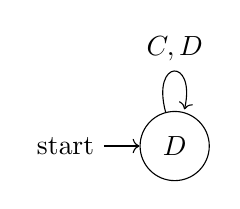
\begin{tikzpicture}[node distance=2cm]
  \node[state,initial] (s_0) {$D$};

  \path[->] (s_0) edge [loop above] node {$C,D$} ();
\end{tikzpicture}
  \centering
  \caption{The always defecting All-D strategy.}
  \label{figurealld}
\end{figure}


    \section{Future Work}
    \label{sectiondiscussion}

    An obvious next step is to prove \cref{pavlovtheorem}. We believe that it should not be too hard. The handwritten notes in \cite{arvid2020} might contain some useful ideas.

    One may also consider other setups. For example, weakening \cref{definitionevolutionarystability} of evolutionary stability by saying that it is only required to not be $\epsilon$-invadable for a fixed $p$, instead of for infinitesimally small $p$, would lead to a more interpretable model. Showing that \cref{evolutionarystable1} still holds in this situation would be interesting.
    
    One can also think of other kinds of noise: for example, a ``failure of the mind,'' which could be modeled by a probability $p$ of being transported to any random state in the automaton. This would automatically make the Markov chain strongly connected, which can potentially simplify a lot of the analysis.


    % \section{Appendix: Time average distributions}

    % We might have periodicity, but for our purposes, we might as well extend the definition and look at periodic distributions as stationary too. The following two lemmas help with that.

    % \begin{lemma}
    %   Given a starting distribution $v$ and a Markov matrix $M$, for every $\epsilon > 0$, there will exist a $k$ such that $|vP^{nk} - vP^{mk}| < \epsilon$ for all $n$ and $m$ $> 0$.
    % \end{lemma}

    % This proves that a Markov chain will always reach a periodic state.

    % \begin{lemma}
    %   Suppose distributions form a chain $p_1 \to p_2 \to \cdots \to p_n \to p_1$. Then $\pi = \frac{p_1 + \ldots p_n}{n}$ is stationary.
    % \end{lemma}

    % This proves that we're able to talk about stationary distributions even when they don't really actually exist.


    % \section{Appendix: Probablistic Automata}

    % OHHHHHHH. THIS WILL HELP WITH MY PROOF????? THIS IS EXACTLY WHAT I'M TRYING TO DO IN MY PROOF RIGHT????? YEAHHHH, NO.

    % In this paper, we have considered strategies that make a deterministic move based on what they perceive. One could also imagine strategies that attaches a certain probability distribution to a perceived input, and chooses their next action based on that. In this appendix we show that these can be reduced to the deterministic ones, and thus that all results for the deterministic ones also hold for the probabilistic ones.

    % Proof idea: we can use cycles in the Markov chain with n total outputs, x of which are to state 1, to model getting to state 1 with probability x / n. this assumes that the outputs are of low enough probability, which can be achieved by chaining together lots of (1-p) transitions, which go to 0.

    % the hard part of this is showing that modifying the finite automaton like this won't hurt us. in fact, it would certainly not hurt us if not every state had to give an output. but that doesn't work for our model i think. so there are certainly things to think about here.



    \bibliography{bibliography.bib}
    \bibliographystyle{acm}


\end{document}